\section{Теоритические сведения}

\begin{wrapfigure}{r}{0.25\textwidth}
    \centering
    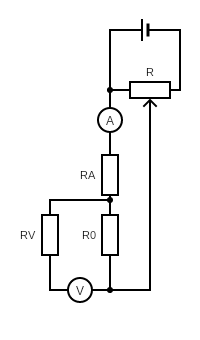
\includegraphics[width=0.2\textwidth]{img/circuit.png}
\end{wrapfigure}

Удельное сопротивление проволоки круглого сечения:
\[\rho=R_0\frac{\pi d^2}{4l},\]
$R_0$~--- сопротивление проволоки, $d$~--- её диаметр, $l$~--- длина.

По закону Ома напряжение $U$ и ток $I$ в образце связаны соотношением
\[U=RI\]

Для измерения тока и напряжения используется схема, изображённая на рисунке.

Вольтметр неидеален, поэтому надо учесть поправку на его конечное сопротивление
$R_V$.

Показания амперметра $I_A$ и вольтметра $U_V$ связаны соотношением
\[V_V=R'I_A\]
$R'$~--- сопротивление параллельно соединённых вольтметра и проволоки.
\[R_0=\frac{R_VR'}{R_V+R'}\approx R'\left(1+\frac{R'}{R_V}\right)\]

График $U_V(I_A)$~--- прямая с наклоном $R'$.
